%% This is file `elsarticle-template-1-num.tex',
%% %% Copyright 2009 Elsevier Ltd
%%
%% This file is part of the 'Elsarticle Bundle'.
%% ---------------------------------------------
%%
%% It may be distributed under the conditions of the LaTeX Project Public
%% License, either version 1.2 of this license or (at your option) any
%% later version.  The latest version of this license is in
%%    http://www.latex-project.org/lppl.txt
%% and version 1.2 or later is part of all distributions of LaTeX
%% version 1999/12/01 or later.
%%
%% The list of all files belonging to the 'Elsarticle Bundle' is
%% given in the file `manifest.txt'.
%%
%% Template article for Elsevier's document class `elsarticle'
%% with numbered style bibliographic references
%%
%% $Id: elsarticle-template-1-num.tex 149 2009-10-08 05:01:15Z rishi $
%% $URL: http://lenova.river-valley.com/svn/elsbst/trunk/elsarticle-template-1-num.tex $
%%

%\documentclass[]{article} %\documentclass[final,3p,12pt]{elsarticle}
%\documentclass[final,12pt,times]{elsarticle}

%% Use the option review to obtain double line spacing
\documentclass[preprint,review,12pt]{elsarticle}

%% Use the options 1p,twocolumn; 3p; 3p,twocolumn; 5p; or 5p,twocolumn
%% for a journal layout:
%% \documentclass[final,1p,times]{elsarticle}
%% \documentclass[final,1p,times,twocolumn]{elsarticle}
%% \documentclass[final,3p,times]{elsarticle}
%% \documentclass[final,3p,times,twocolumn]{elsarticle}
%% \documentclass[final,5p,times]{elsarticle}
%% \documentclass[final,5p,times,twocolumn]{elsarticle}

\usepackage{amssymb}
\usepackage{wrapfig}
\usepackage{lipsum}
\usepackage{natbib}

\usepackage{tikz}
\usetikzlibrary{shapes, arrows}

\tikzstyle{notary} = [rectangle, draw, text centered, text width=4em, fill=blue!20, minimum height=2em]
\tikzstyle{user}   = [rectangle, draw, text centered, text width=4em, fill=green!20, minimum height=2em]
\tikzstyle{server} = [rectangle, draw, text centered, text width=4em, fill=red!20, minimum height=2em]
\tikzstyle{single}   = [draw, -latex']
\tikzstyle{double}   = [draw, latex-latex']

% http://tex.stackexchange.com/questions/35712/modify-footer-used-by-elsarticle-cls
\makeatletter
\def\ps@pprintTitle{
    \let\@oddhead\@empty
    \let\@evenhead\@empty
    \def\@oddfoot{\centerline{\thepage}}
    \let\@evenfoot\@oddfoot}
\makeatother

\journal{University of Guelph; CIS*4110}

\begin{document}

\begin{frontmatter}

\title{Exploring the removal of centralized authories from SSL}


\author[doug]{Douglas Anderson}
\author[eric]{Eric Boyd}
\author[james]{James Kelly}
\address[doug]{dander01@uoguelph.ca}
\address[eric]{boyde@uoguelph.ca}
\address[james]{kellyj@uoguelph.ca}


\begin{abstract}

    So abstracts are pretty cool and stuff. Good ones have information about
    the project. This one does not.

\end{abstract}

\begin{keyword}
% keywords here, in the form: keyword \sep keyword
Security \sep
SSL \sep
Central Authorities
\end{keyword}

\end{frontmatter}

\section{Introduction}
\label{intro}

In the modern world the Internet holds a very important role in commerce and
social aspects of life. Both of these pursuits require the ability for two or
more parties to communicate securely. To facilitate this secure communication,
the Internet has resorted to using the SSL (Secure Socket Layer) and it
successor TLS (Transport Security Layer) to protect the data being exchanged.
These protocols utilize public-private key pairs to facilitate RSA encryption.
While this protocol has been extremely successful it must rely on a central
authority to confirm the identity of the owner of public keys. This central
authority is a single point of failure in this authentication system, and has
in the past been compromised, allowing successful impersonation of several
popular, high profile websites.

In 2011 the central authority Comodo Group, Inc. was hacked and the hacker made
off with a SSL certificates for various sites including Gmail, Yahoo Mail,
Hotmail.  \citep{comodohack} This would allow the hacker to preform man in the
middle attacks on the sites and read the emails of users of these services. The
attack was easily executed because of Comodo's extremely weak password that was
easily broken with a word list. This illustrates the vulnerability in the SSL
protocol that central authorities create.

\section{Background}
\label{Background}

%TODO write about how SSL works
%TODO write about how CAs work
%TODO write about how Perspectives work

\begin{figure}[h]
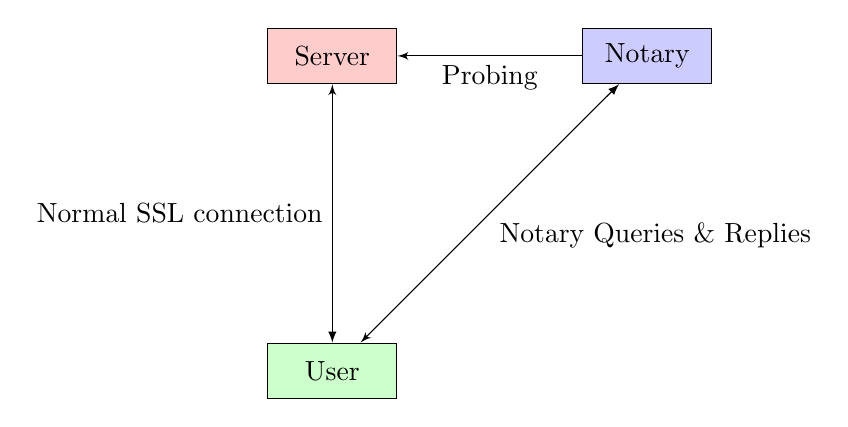
\begin{tikzpicture}[node distance = 4cm, auto]
    \node[server](server){Server};
    \node[notary, right of=server](note){Notary};
    \node[user, below of=server](user){User};
    \path[double](note) -- node {Notary Queries \& Replies}(user);
    \path[double](user) -- node {Normal SSL connection}(server);
    \path[single](note) -- node {Probing}(server);
\end{tikzpicture}
\caption{Normal Performance of the perspectives system.}
\end{figure}

\section{Method}
\label{Method}

For our project we attempted to build upon the Perspective Project by allowing
servers to send messages to notaries requesting that the notary make note of
the change of SSL certificate. This fixes the problem in the perspectives
project that can occur when a server changes it's SSL certificate and a user
queries the notary for that server's SSL certificate. Because the notary has
not yet updated it's record of the SSL certificate and reports to the user that
there is a mismatch which may lead the user to abort their attempt to create an
SSL connection.

\begin{figure}[h]
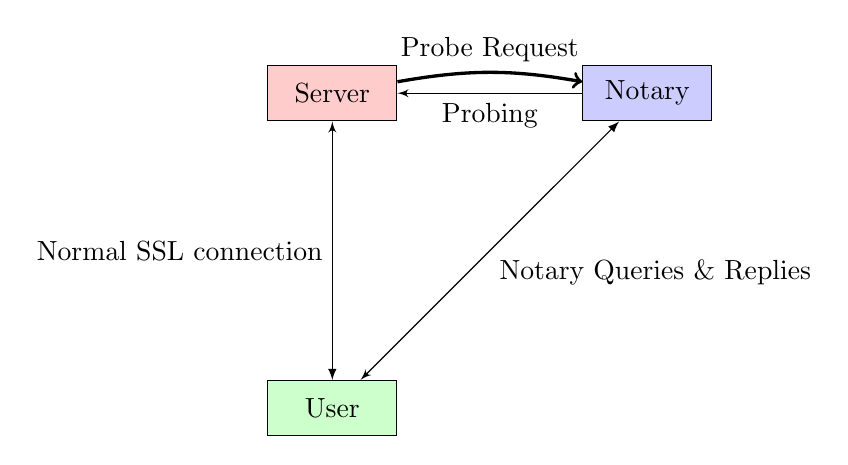
\begin{tikzpicture}[node distance = 4cm, auto]
    \node[server](server){Server};
    \node[notary, right of=server](note){Notary};
    \node[user, below of=server](user){User};
    \path[double](note) -- node {Notary Queries \& Replies}(user);
    \path[double](user) -- node {Normal SSL connection}(server);
    \path[single](note) -- node {Probing}(server);
    \path[->](server) edge[very thick, bend left=10] node{Probe Request}(note);
\end{tikzpicture}
\caption{Our modified perspective notary allows for the server to request that
    it's SSL certificate be probed and updated in the Notaries Database.}
\end{figure}

\section{Results}
\label{results}

\section{Conclusion}
\label{conclusion}

\section{Further Work}
\label{further work}

\section{References}
\label{references}
\nocite{*}
\bibliographystyle{plainnat}
\bibliography{report}

\end{document}

